\chapter{Introduction}%
\label{chapter:introduction}

\begin{introduction}

\end{introduction}

\section{Concept}\label{sec:concept}

\subsection{Basketball Context}\label{subsec:basketball-context}
Portugal is cleary not known for its basketball, the quality is far behind other european countries.
In the International Basketball Federation (FIBA) world ranking\cite{fiba}, Portugal is in the 47 place, and in the middle of the European table in 25th place.
Comparing with our neighbours Spain that is in 7th in the world ranking.
However, in the past years, the portuguese basketball achieve some marks.

First, Portugal had its first player in one of the best women league in the world, ``Ticha'' Penicheiro played during 15 seasons in the WNBA in th USA, winning a title with the Sacramento Monarchs, and some individual awards.
And in 2019, entered the Women’s Basketball Hall of Fame, that has the goal of honouring the most influential players in women basketball.\cite{ticha}

After her, Neemias Queta was drafted to the NBA in 2021, being the first portuguese in the NBA, and in the 2023--24 season won his first title with the Boston Celtics.
Besides not being the most valuable player in his team in the USA, he played an important role with the National team in second appearance in the EuroBasket tournament in 2025.
In this campaign, the portuguese team made a surprise performance, passing through the group phase and then, confronting the German team.
In this game the portuguese team was holding up until the last quarter, where the world champions and the winners of the EuroBasket 2025 took the victory.
After the first victory in the EuroBasket, Neemias mentioned that it was a great moment fot the sport in Portugal and wants the sport to grow more in Portugal.\cite{neemias}
To help with this goal, a survey was made in order to understand how players and basketball enthusiasts use the public basketball courts, the frequency, and the problems.

\subsection{Problem}\label{subsec:problem}

After a some conversations with few basketball players and leaning heavily in a survey responses, basketball players and enthusiasts wish to go more often to public courts.
Besides time constraints, this two scenarios and the following complains are in these players mind:

\paragraph{Key Scenarios}
\begin{itemize}
    \item \textbf{Insufficient players}: people arrive to play but cannot form a team because not enough players are present;
    \item \textbf{Overcrowding}: courts are full, forcing players to wait or leave.
\end{itemize}

\paragraph{Common annoyances reported}
\begin{itemize}
    \item Poor or unpredictable court conditions;
    \item Courts that are either empty or overcrowded;
    \item Social problems between players, including aggressive or unpleasant behaviour, individualistic style, and mismatched competitiveness (players who do not take the game seriously or whose skill and attitude creates a poor experience).
\end{itemize}

These issues point to a coordination and information problem.
Basketball players lack a platform to discover, schedule and evaluate informal games, and to verify court availability and condition.
As a result, players often waste time visiting courts with unsatisfiable condition, which decreases participation and lower quality of both social and sporting experience.

\subsection{Proposed Solution}\label{subsec:proposed-solution}

The proposed solution is to design and implement a digital platform that addresses the coordination and information gaps in amateur basketball in public courts, by focusing on two primary features:

\begin{description}
    \item [Informal Games] ``Pickup games''\footnote{``Pickup games'' is the name used by basketball players to call a game without a formal organization (not in a league, no referee, no strick rules)} -
    Enable players to create, discover and join informal matches (pickup games), with features that support different play modes and social organization:
    \begin{itemize}
        \item Players can create, search for and join games listed on the platform;
        \item The games can be competitive or casual;
        \item Competitive games contribute to a leaderboard/raking table per court;
        \item Game formats include 1v1, 3v3, 4v4, 5v5;
        \item Users can create and mange persistent teams and challenge other teams;
        \item Users can set a team as ``next''\footnote{``next'' is used in the casual pickup games to tell the current teams playing, that wants to play against the winning team.} to a game, to play against the winner.
    \end{itemize}

    \item[Court Availability and condition awareness]
    Provide users with real-time and information about courts so they can decide where and when to play:
    \begin{itemize}
        \item Persistent court catalogue with attributes - name, location, full/half court, number of courts, has water fountain, etc;
        \item Users can indicate intent to attend a court at a specific time, so others can have an idea of the availability;
        \item User can mark themselves ``present'' at a court;
        \item Optional automatic geolocation-based check-in to simplify presence signalling;
        \item Live occupancy indicators to show how many users intend to go and how many are currently present;
        \item Court condition reporting by the users, they can submit short status updates to report issues.
        \item Display short weather summary for the court location (optional)
    \end{itemize}
\end{description}


\section{State of the Technology}\label{sec:state-of-the-technology}

This platform has to reach the maximum basketball players for it to work properly, and should work when the players are in the court, or anywhere.
In order to achieve this, the platform should be access from the mobile phones, and Statcounter\footnote{Statcounter is a company that provides a tool for users to get insights of their website's visitors} Global Stats reports the following about the Mobile Operating System Market Share in Portugal in September 2025: 65.65\% is from Android, and 33.94\% is iOS\cite{statcount}.
Despite the fact that more than half of people uses Android, the goal is still reach the maximum players possible, so the platform should be accessible from Android and iOS phones.

In order to develop a mobile application for both platforms, there are different options of approaches that can be selected for the implementation, which are the native, cross-platform, web, hybrid, modeling, cloud-based and merged approaches\cite{Khachouch2020}.

\subsection{Native Apps}\label{subsec:native-apps}

Going Native, means that the app will be developed with to a specific OS, using its programming language.
To build native Android applications, developers typically use Kotlin or Java.
Both language are compiled to Java Bytecode that runs on the Android Runtime (ART).
As for iOS, developers use Swift or Objective-C, mainly the first one, to build native iOS applications.

With native apps, there is no need for third-party frameworks, as the code is compiled directly into the platform's native language.
This results in better performance and faster execution compare to other solutions, which will be discussed later.
In addition to performance, native development offers security benefits, since developers can take advantage of the built-in security features of the operating system.
When it comes to  User Interface (UI) and User Experience (UX), each platform provides its own guidelines: Android follows Material Design, while iOS follows Human Interface guidelines.
This consistency makes apps easier to navigate, and there is no issues in the app adaptation to other devices.
Finally, native applications can make full use of device features such as the camera, microphone and GPS, which enhances functionality and integration.\cite{Nagy2022}

When the goal is to deliver an application for both Android and iOS using native development, each feature must be implemented twice, once for each platform and in different programming languages.
As Roby Nagy explains in \textit{Simplifying Application Development with Kotlin Multiplatform Mobile}\cite{Nagy2022}, the development cost of this approach can be expressed as:


\[Cost of development (n) = n * FC\]

where \textit{n} represents the number of platforms and \textit{FC} the \textit{feature complexity}, defined as the sum of all sub-features that compose a feature.
The figure~\ref{fig:costNative} , taken from Roby Nagy' book\cite{Nagy2022}, illustrates how the development cost grows for two platforms (blue line) and three platforms (red line) as the number of features increases, assuming no cost reduction from sharing code.

\begin{figure}[h]
    \caption{Cost of native development as a function of feature comlpexity \cite{Nagy2022}}
    \centering
    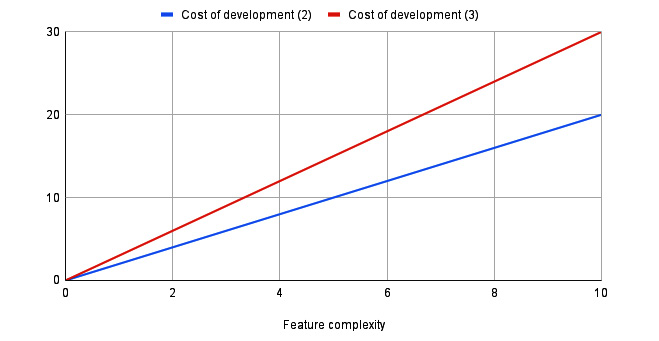
\includegraphics[width=0.5\textwidth]{figs/Figure_1.1_B17614_cost_of_native_dev}
    \label{fig:costNative}
\end{figure}


Beyond this calculation, additional factors complicate native development.
Each platform has distinct characteristics, and a solution that is straightforward to implement on one platform may be unavailable or significantly harder to achieve on another.
This divergence creates extra overhead in aligning features sets across platforms.
So, Nagy introduces the additional component, \textit{Synchronization Cost}, which increases in an exponential way as the number of features and its complexity grows.
The updated formula is expressed as:

\[Cost of development (n) = n * FC + Sync Cost ^ {FC}\]


\subsection{Web Applications}\label{subsec:web-applications}

Any application that is access through \textit{HTTP} requests over a network is called a web based application.
These applications are implemented with HTML, CSS and JavaScript.
Until Progressive Web App appeared, these applications were browser only, but now, they can be installed in the device, can have offline availability, push notifications and background sync, also able to run on desktop.
Developers normally use Angular or React, and other frameworks are StencilJS or Svelte.
However, PWAs cannot access key platform's features as the Native apps can, and also, has a possible higher energy consumption.\cite{Huber2021}


\subsection{Hybrid Applications}\label{subsec:hybrid-applications}

Another option, also leveraging web technologies such as HTML, CSS and JavaScript, is taking a hybrid approach.
The app is developed with as web app and developers wrap the app via cross-platform wrappers, frameworks and tools, as a native app.
With this approach, the app as a user experience just as a native app.
Some hybrid app frameworks are Cordova, Phonegap, Titanium, Ionic, being the first the most common.
Using third-party plugins with JavaScript, it is possible to access features form the device, such as the camera and GPS\@.
In the Maher Gerges and Ahmed Elgalb article\cite{Gerges2024}, where they compare different approaches, it is compared the hybrid apps directly with the native apps, and, in CPU and Memory occupancy, the hybrid cost more, being 106\% higher and 73.0\% higher in order.
Also, not all features are available and the performance is worse than native apps.\cite{Gerges2024}


\subsection{Cross-Platform Apps}\label{subsec:cross-platform-apps}

In order to avoid repeating the same code for different platforms, there are Cross-Platforms approaches.
With this method, it is possible to create applications that run on multiple operating systems.
In a first look, using cross-platform methods can be an effective solution to develop applications for a multiple platforms, when time, cost and basic interoperability is the primary concern.
On the other hand, Cross-Platform applications tend to have the worst performance and user experience compared with Native apps, as they are behind the evolution of Android and iOS and cannot take full advantage of each platform's features\cite{Nagy2022}.
In different articles and papers, the categorization of the approach varies, especially, when it comes to the Cross-Platform approach, there are subcategories\cite{ELKASSAS2017163}.
The Web and Hybrid approach is normally inserted in this category, alongside with Interpreted approach and Cross-Compiled approach\cite{ELKASSAS2017163}, which the most popular used frameworks are React Native and Flutter, respectively.

\subsubsection{Interpreted Approach - React Native}

Similar to the web and hybrid approach, uses web technologies such as CSS and JavaScript, however, the user interface is not HTML and not render in the browser.\cite{Huber2021}
The most popular used framework is React Native from 2015, developed by Meta, where developers build applications with React components, and the logic in JavaScript.
This framework uses component-based architecture, following the steps of React for the web, promoting code reusability, modularity and easy debug.\cite{10667693}
The JavaScript code executes on a separate thread and communicates with the native layer through a bridge\cite{Nagy2022}, allowing developers performance-critical parts of the app in native languages\cite{10667693}.
The bridge translates asynchronous, serializable data between the two environments, which enables native rendering of components.
However, this approach introduces overhead, resulting in a process generally slower compared to fully native applications.\cite{Nagy2022}

\subsubsection{Cross-Compiled Approach - Flutter}

In this approach, the app is developed in a common language, and then, it is compiled to the native code that can be executed on a mobile device, with Flutter and Xamarin popular examples.\cite{Huber2021}
Flutter is a framework developed by Google, its architecture can be described in three layers, as noted by Roby Nagy in his book\cite{Nagy2022}.
The Framework layer, where developers write the application code and the UI components, declaratively using the Dart language.
The Engine layer renders Flutter widgets to a canvas called Skia Canvas, which is then passed to the final layer, the native platform.
The platform displays the canvas and sends back user events to the framework.\cite,{Nagy2022}
Compared to React Native, Flutter often achieves better performance by relying on Android's Native Development Kit and iOS's Low-Level Virtual Machine to compile code coming from the engine, Flutter applications deliver higher execution performance.
Nevertheless, certain parts of a Flutter application may still need to be implemented in Java/Kotlin and Obj-C/Swift code.
Communication between these native components and the Dart code is through a channel, reducing scalability\cite{Nagy2022}.

\subsubsection{Cloud-based Approach and Modeling Approach}

A Cloud-based application, has its backend in the cloud, instead of running locally, using the cloud features such as flexibility, virtualization and security.\cite{ELKASSAS2017163}
Companies like Amazon Web Services, offer that service called Backend as a Service (BaaS).\cite{Khachouch2020}

There are two subcategories in this approach, the Model-Based User Interface Development (MB-UID) and the Model-Driven Development (MDD).
Developers use abstract model to describe tasks, data, users and the user interface, which will generate source code.
It can transform to code from different platforms.
Some tools include XMobile, for MB-UID and JavaScript Application Framework for MDD\@.

\subsubsection{Cross-Platform vs Native}

So, on one hand, using cross-platform frameworks can be an effective solution to develop applications for multiple platforms, when time, cost and basic interoperability is the primary concern.
On the other hand, these frameworks tend to be behind the evolution of Android and iOS, and cannot take full advantage of each platform's features.
Roby Nagy therefore refines the development-cost equation as:

\[Cost of Development (n) = FC * (1 + Cost of going Native)\]

In this equation, \textit{n} is the number of platforms and \textit{FC} is the feature complexity.
As for the \texttit{Cost of going Native}, reflect the additional effort required when some parts must be implemented with native code.
Its value depends on the level of interoperability that the cross-platform framework provides with native components, which is not optimal.
When there is a necessity to implement native code, the knowledge gap between the framework and native languages adds to the expense, as well as the synchronization.\cite{Nagy2022}\\

With this, it is possible to visualize the different cost of development, adding the Cross-Platform with roadblocks.
The figure\ref{fig:costNative}, illustrates how the cost of cross-platform development increases relative to both cost of Native and Native with Sync Costs.
A roadblock occurs when a required feature cannot be implemented only with the frameworks and must instead be written in native code, producing a sudden rising in cost.
If no native features are required, cross-platform development can remain less expensive with the previous discussed limitations.
However, as more features demand native implementation, the cumulative cost eventually exceeds that of a fully native approach.\cite{Nagy2022}

\begin{figure}[h]
    \caption{Cost of cross-platform development with potential roadblocks as a function complexity\cite{Nagy2022}}
    \centering
    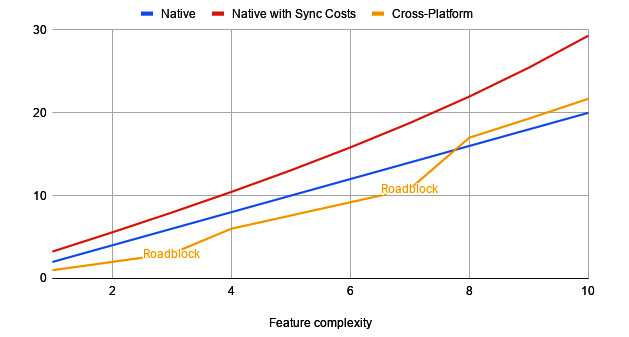
\includegraphics[width=0.5\textwidth]{figs/Figure_1.6_B17614_cost_of_cross}
    \label{fig:costCross}
\end{figure}


\subsection{Kotlin Multiplatform}\label{subsec:kotlin-multiplatform}

Although cross-platforms the previous frameworks solve the problem of dealing with different platforms, it is still not optimal if the application demands platform specific features, and keeping up with Android and iOS updates.
To go around these conditions, developers can choose Kotlin Multiplatform (KMP), also a cross-platform solution.
As Jetbrains mentions in their website, Kotlin Multiplatform is an open-source technology developed by JetBrains, that allow developers to create applications for multiple platforms in an efficient way, by reusing code across them and still having the native approach benefits.[cite:@kmpJetbrain]
Developers can share code without losing the qualities of native programming, have good user experience, good app performance and having full platform capabilities, alongside the benefits of the cross-platform, reducing development time, consistency in behavior in the different platforms.
In this approach, the developer has 3 options, it can share and only write a critical feature in Kotlin, or implement the full logic and only develop the UI natively, and finally, with Compose Multiplatform, also share the UI.\cite{kmp}

Jetpack Compose\cite{jetpack} is a toolkit to develop the User Interface of Android apps.
It is implemented in a declarative way, compatible with Kotlin APIs, enabling developers to intuitively build fast UIs.
It also supports Google's Material Design, an ``open-source design system for building beautiful, usable products''\cite{materialD}.
Since 2021, developers can build shared UIs for Android, iOS, desktop and web, feeling natural on every platform with Compose Multiplatform.\cite{compose-multi}

Thompson Carter, refers in his book\cite{kotlinInDepth} the same benefits of KMP, code reusability, faster development, reduce maintenance (as it is only need to fix bugs in one place), flexibility (share code and still access platform-specific features and APIs) and community support.
However, he mentions some challenges as:
- Maturity, as the KMP is recent and is still evolving, some libraries and tools may not be fully supported;
- The integration with Platform-Specific APIs can be challenging;
- The transition from single-platform development can be a bit difficult, with the introduction of new paradigms;
- And the integration with an existing project can involve significant refactoring.

\subsection{Overview}\label{subsec:overview}

The table\ref{tab:approaches-comprehensive} syntheses the characteristics of the mobile development approaches .

\newcolumntype{Y}{>{\raggedright\arraybackslash}X}

\renewcommand{\arraystretch}{1.2}
\setlength{\tabcolsep}{8pt}

\begin{table}[ht]
    \centering
    \caption{Comparison of mobile application development approaches; \cite{Khachouch2020, 10667693}}
    \label{tab:approaches-comprehensive}
    \small
    \begin{tabularx}{\textwidth}{|p{3.2cm}|Y|Y|Y|}
        \hline
        \makecell[l]{Approach / \\ Framework} &
        \makecell[l]{Advantages} &
        \makecell[l]{Disadvantages} &
        \makecell[l]{Best use cases} \\
        \hline

        Native apps &
        Best performance; full access to platform APIs and sensors; highest UX fidelity; mature tooling and debugging. &
        Two codebases for multiple platforms with higher cost &
        When maximum performance, platform-specific UX or deep hardware access are required. \\
        \hline

        Web apps / PWAs &
        Single codebase; runs on desktops and mobile browsers; easy distribution via web. &
        Limited access to some native features; performance and energy use vary vs native; &
        When reach and ease of deployment matter; suitable for simple apps or when minimal native features are needed. \\
        \hline

        Hybrid (wrapped web) &
        Faster port from an existing web app to an installable app; single web codebase; plugin ecosystems to access device features. &
        Worse performance than native; higher CPU and memory usage; some native features may be unavailable; UX can feel non-native. &
        Quick conversion of existing web apps into installable apps; prototypes and low-budget MVPs. \\
        \hline

        React Native (interpreted) &
        High code reuse; React ecosystem; UI renders using native components; faster than pure WebView hybrids for UI responsiveness; good developer velocity. &
        Bridge overhead can reduce performance for heavy UI/CPU work; some features require native modules; platform parity depends on third-party library support. &
        Apps with standard UI and business logic where development speed and native look are both important. \\
        \hline

        Flutter (cross-compiled) &
        Compiled to native code (via Dart); high performance; consistent UI across platforms via Skia; rich widget set enabling polished UIs. &
        Larger binary sizes; occasionally needs platform channels to access native features; different paradigm (Dart and Flutter widgets) for developers. &
        When near-native speed is wanted and a single codebase with highly consistent UI across platforms. \\

        \hline

        Kotlin Multiplatform (KMP) &
        Share core business logic (networking, storage, domain rules) across platforms; retain native UIs or use Compose Multiplatform; near-native performance and good interoperability with native code. &
        Ecosystem still maturing; some libraries may be platform-limited; complex when integrating with existing native projects; tooling and third-party support are improving. &
        When  substantial logic reuse is wanted while keeping native UI/UX and performance; especially attractive for Kotlin-centric teams. \\
        \hline
    \end{tabularx}
\end{table}


\subsection{Competitor Research}\label{subsec:competitor-research}

After getting an idea about what are the problems in the portuguese bass made through what is in the market that could solve the main issues.
For this research, different approach were taken to find results.
Below is shown the approach and the results, and then, the results will be analysed deeper.


\subsubsection{Search}
By searching the browser using the query ``Play basketball in Portugal'', the useful links found for someone who just want to go to a public court and play some casual games, or shoot some balls, where from a website called ``Courts of the World''\cite{fiba-courts}, ``Meetup''\cite{meetup}, a question in Reddit from 2021\cite{reddit}, a blog called ``World Baller''\cite{worldBaller}, and some websites for clubs and schools.
With the query ``Basketball pickup games portugal'', the results were similar, with the AI from the browser telling to look for games in Facebook groups, in Meetup, and suggested 3 courts in Lisbon.

Using Perplexity AI, using this prompt in a deep research ``I am from Lisbon and  I play basketball.
I would like to go play on the weekend in a public court.
Where can I go?
Is there any platform I can find some casual games to join?''\cite{perplexity}, the model provided 4 public courts with a description, for example:

``Campo de Laranjeiras ("The Blue Court") near Laranjeiras Metro features two full courts with fresh surfaces and multiple hoops.
Locals refer to it as the "blue court" due to its bright surface color.
It has a semi-competitive vibe with frequent rotation of players and is open 24/7 with free access.''

Besides that, it provided information about a group in Meetup, and a facebook group.
As for platforms, it indicated an app that does not available in Portugal, called ``Pickup: Connect \& Play Sports'', another called ``Pickup Sports (Adult League)''\cite{pickup-adult}.
Then it also shows ``Courts of the World'', that has an iOS application, and another app called ``Fullcourt: Pickup Basketball''\cite{fullcourt-pp}.

Using ChatGPT, with the same prompt, with the free version and the option of \textit{Web Search} activated, it answered with 8 public courts, with the Meetup group already mention above, as well as the facebook group, and the blog ``World Baller''\cite{chatgpt1}.
With the \textit{Thinking} option it provided some courts with the reference to ``Courts of the World'' website and the reddit question from above.
It also provided the same platforms, and gave some tips\cite{chatgpt2}.

Another query made in the browser to explore ways for players to play casual basketball was ``\textit{reservar campos de basquetebol portugal}'' \footnote{book basketball courts portugal}, where it shows some private places to book, and a platform called ``AirCourts''\cite{aircourts}, that gathers different courts from different sports to help users book them.
In the website of AirCourts it was saying that they will join ``Playtomic''\cite{playtonic}, that is a platform to book courts and find players in padel and tennis.

In another search, ``\textit{Torneios amadores portugal basketball}''\footnote{Amatour tournments portugal basketball}, only one result from the first page would be useful for someone who wants to play casual basketball games, the website ``Jogabasket''\cite{jogabasket}.

Going to the Google's Play Store, and searching for ``Pickup'' apps, several appeared, which Perplexity AI already mentioned, as well as, ``Pickup: Play \& Host Sports''\cite{pickup, pickup-app}, ``GoodRec''\cite{goodrec} (it is not available in Portugal), ``WOOOBA''\cite{woooba} and ``Pick-Roll''\cite{pick-roll}.


\subsubsection{Existing Options}

\textbf{Courts of the World}\cite{fiba-courts} - Is a FIBA endorsed platform, available in web and in iOS, where users can find courts around the world.
In the home page, the users can search for a place or click a button to view basketball courts near the user, which did not work when searching for Lisbon or Porto and even clicking in the button, it was loading for a long time.
There is a section called ``The World’s Favorite Basketball Courts'' that shows cards with famous courts.
In the menu is the option to list the courts, that has list of countries divided by continent.
Going to Portugal, it appears the most popular courts.
Opening the first court in the most popular, ``Campo Dos Mártires Da Pátria'', there user can view on the map (which does not work), rate the court, this one having 8 ratings, an option to check in, saying the player is there, and the platform asks for the location to confirm, and it is saying that 1 player checked in last 5 years ago, and the user can save the court, with 7 players saving.
Besides that, there are some photos of the court, with the last uploaded November 2024 (at the date), and any player can upload media.
Players can add information about the court and see local insights, such has the weather conditions.
In the platform, there is also a blog and a section of the players, with a leaderboard of players that contribute for the platform, with courts added, photos and comments.
This looks like a good option for players to find courts, and it looks like it has a feature of check in, so other players can see how full is the court.
However, it looks like there is not much adherence on the part of the players

\textbf{Jogabasket}\cite{jogabasket} - From the part of the Portuguese Basketball Federation, this website has the same purpose as the Courts of the World.
In the home page, the user can find clubs, by searching a location, showing clubs as the result and their contacts.
Scrolling down, the user can find some courts around Portugal, with map that works perfectly.
There is also a section to find 3x3 tournaments, but, at the time of writing, there is nothing there.
Finally, there are some images of the courts.
This website is good for users to find courts in Portugal.

\textbf{Meetup}\cite{meetup} - This platform is not only for sports, here users can find groups for any type of activity, and, inside the group, the host can create events.
There is a group called ``Lisbon Basketball Club''\cite{meetup-basketball-group}, that run indoor games every Monday and Sunday, paying a fee to book the court.

\textbf{Pickup Sports (Adult League)}\cite{pickup-adult, pickup-adult-app} - Is an app for Android and iOS where users can find leagues of more than 15 sports, including basketball.
Looking in the website\cite{pickup-adult}, in the ``How it works section'', it says to pick the sport, select a city and an area and find a games.
For basketball, it is saying in the website that users can join competitive leagues, or just pick up games with friends.
Opening the app, the user needs to create an account in order to search for games.
However, the search was confusing, after choosing the location, it looked like it went back to the default, Los Angeles.
Choosing the sport, basketball, it did not appear any game.
It is possible to see a list of players, but just a few, and they are all form Los Angeles.
Also, it is possible to see how many games the players went, but only one player had one game.
It looks like the app is not used, specially in Portugal.
In the app as a earning system, a user can create games and charge other users, earning seventy-five percent of the revenue, the rest must be going to the app.

\textbf{Fullcourt: Pickup Basketball}\cite{fullcourt, fullcourt-pp} - Is a platform to organize basketball pickup games.
When creating an account, the user sets its height, wight and vertical.
Then, the position, the skill level and the frequency that it plays.
In the app, the user can create quick games, by inviting nearby players, selecting a court and hours.
After creating, the players receive an invitation and can select if they are attending.
In the game detail view, it shows who is going and the position the player plays, who is not going and who is still to accept, besides that, it has a chat.
In the courts view, there is a map that shows the number of players in the area, and upcoming ``Runs'', which is a weekly recurring game at the same time and location.
Going to Lisbon, there are in total 10 users, and one court in the map.
In the profile view, it is available the win/lose record, showing the number of vitories and losses, the number of games and the percentage.

\textbf{``Pickup: Play \& Host Sports''}\cite{pickup, pickup-app} - Is a platform to host and join games for various sports.
When creating an account, the user chooses the sports and the level he plays.
In the home page, the user can search games, enter a game code, and there is a dashboard, which is not showing anything, probably being games nearby, and this current location (Lisbon) it does not have games.
There is also another view with a search bar, to search for games, sport and locations.
However, it is not showing any game, as it is most likely to not existing in Portugal.
There is also a feature that is communities, existing only sixteen and in Hong Kong, where there is a public chat and games for the members to join.
Finally, it is possible to create games, choosing the sport, the level, if it is a public court or public, indoor or outdoor, individual or team game and if it is public or private.
Then, select the time, the game duration, and the number of players, or teams (including the team size).
After creating a game, it did not appear anywhere in the app.
There is a function to create a team, that can join the games.

\textbf{WOOOBA}\cite{woooba} - Is another platform to create and join basketball games.
When crating an account, the user can choose the position and also being a referee.
The user can select the age, and the skill range, and also set who can see the profile.
Anyone can create games, and they can be free or paid, and the app takes a fee when it is paid.

``Pick-Roll''\cite{pick-roll}
``AirCourts''\cite{aircourts},
``Playtomic''\cite{playtonic}














































